\section{Roadmap du sprint Pre-Developpement}

Avant de nous lancer dans la programmation, nous avons souhaité bien poser les bases. L’objectif de ce sprint est de:
\begin{itemize}
    \item Comprehension du problème que nous souhaitons traiter, notamment par la recherche de la documentation existante sur
     le sujet et par l'établissement d’un cahier des charges clair
    \item Définition de la méthodologie de développement et de l’organisation au sein de l'équipe
    \item Mise en place des outils nécessaires au bon fonctionnement futur
\end{itemize}


Pour ce faire nous avons entrepris plusieurs tâches qui se résument de la manière suivante:

\begin{center}
    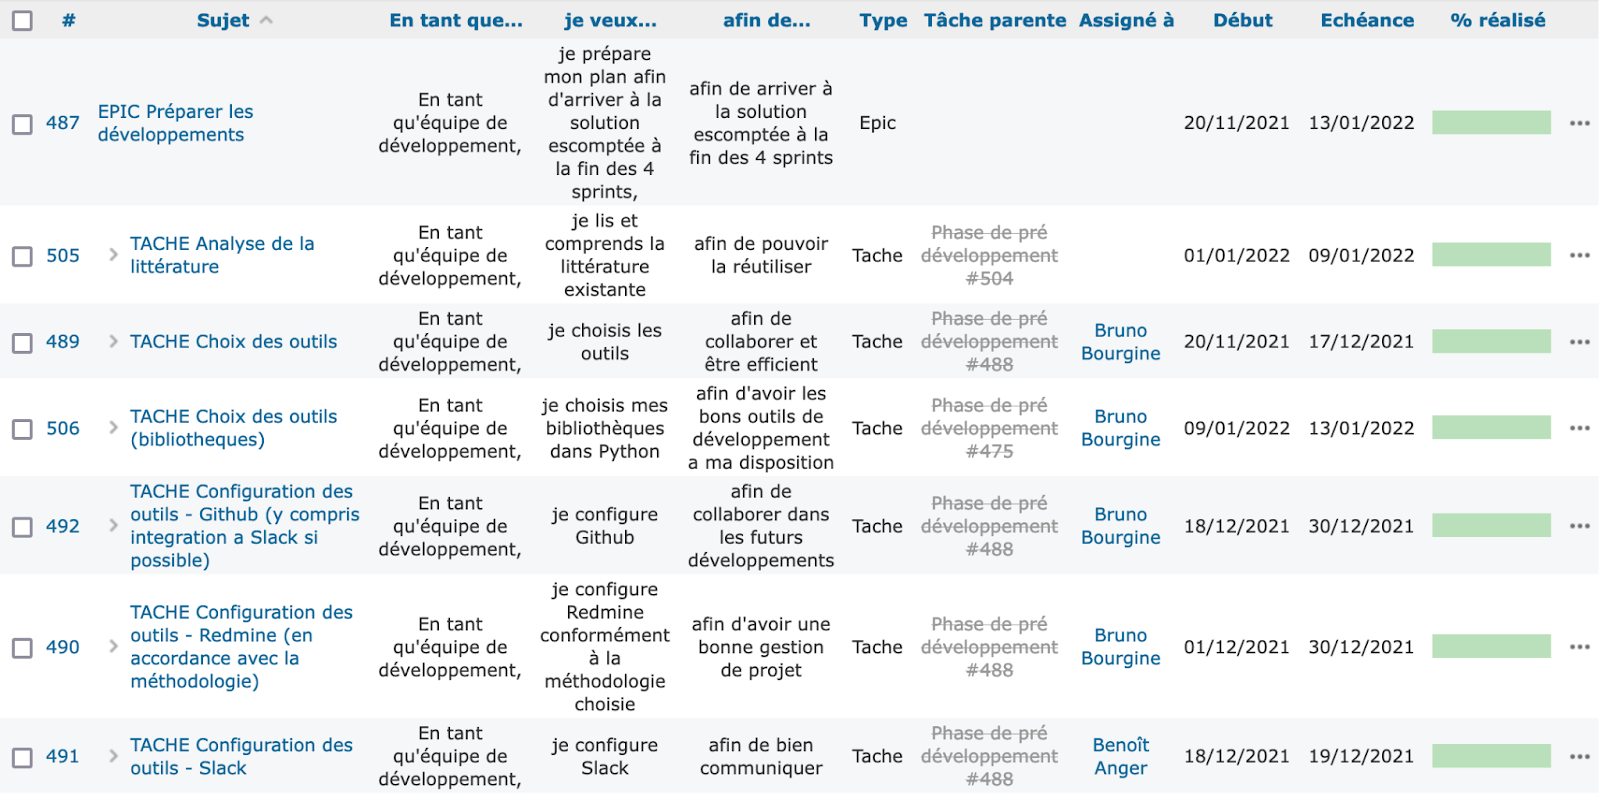
\includegraphics[width=17cm]{images/roadmap-predev-part1.png}
\end{center}

\begin{center}
    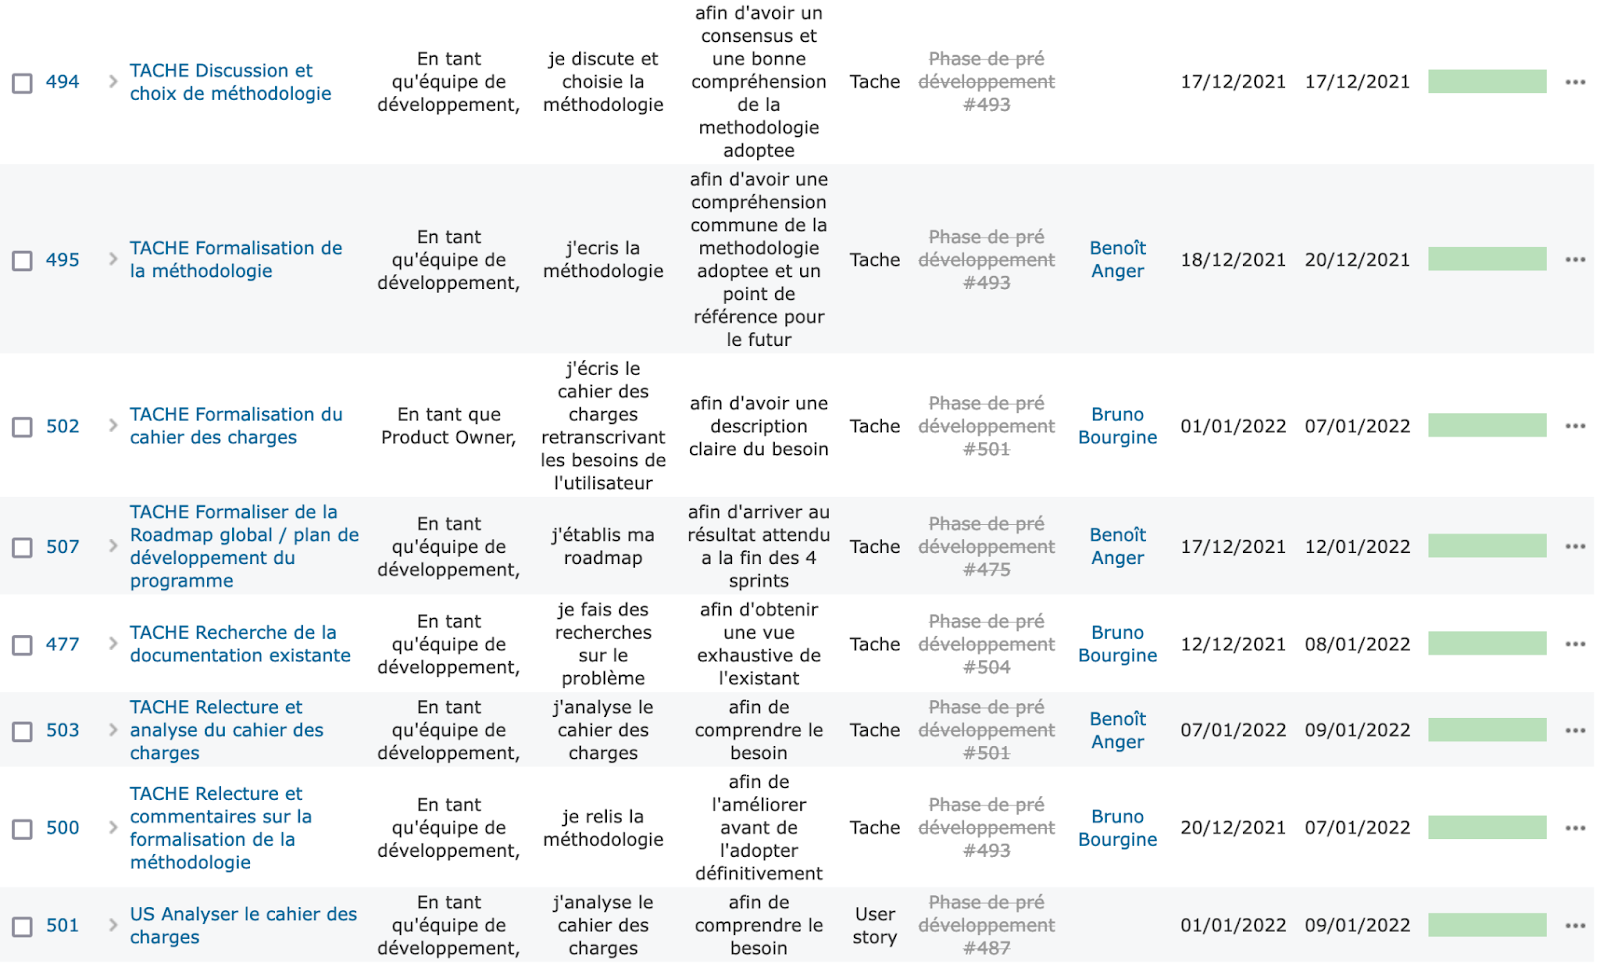
\includegraphics[width=17cm]{images/roadmap-predev-part2.png}

    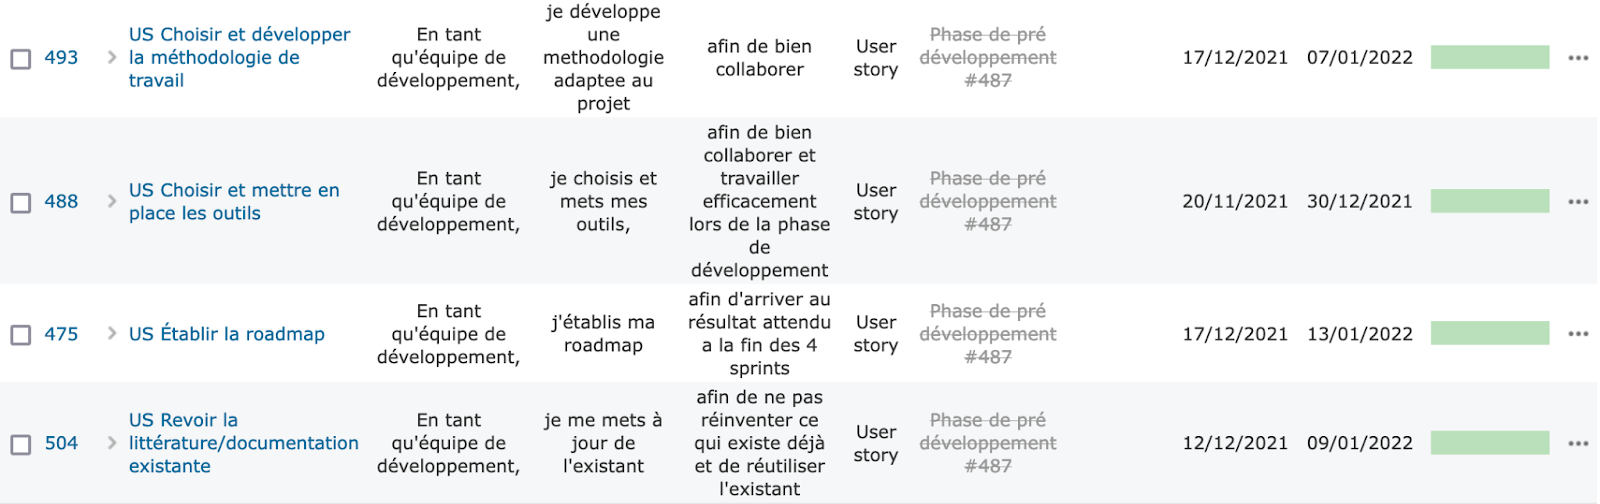
\includegraphics[width=17cm]{images/roadmap-predev-part3.png}
\end{center}

\newpage
Et ici présenté en diagramme de Gantt:

\begin{center}
  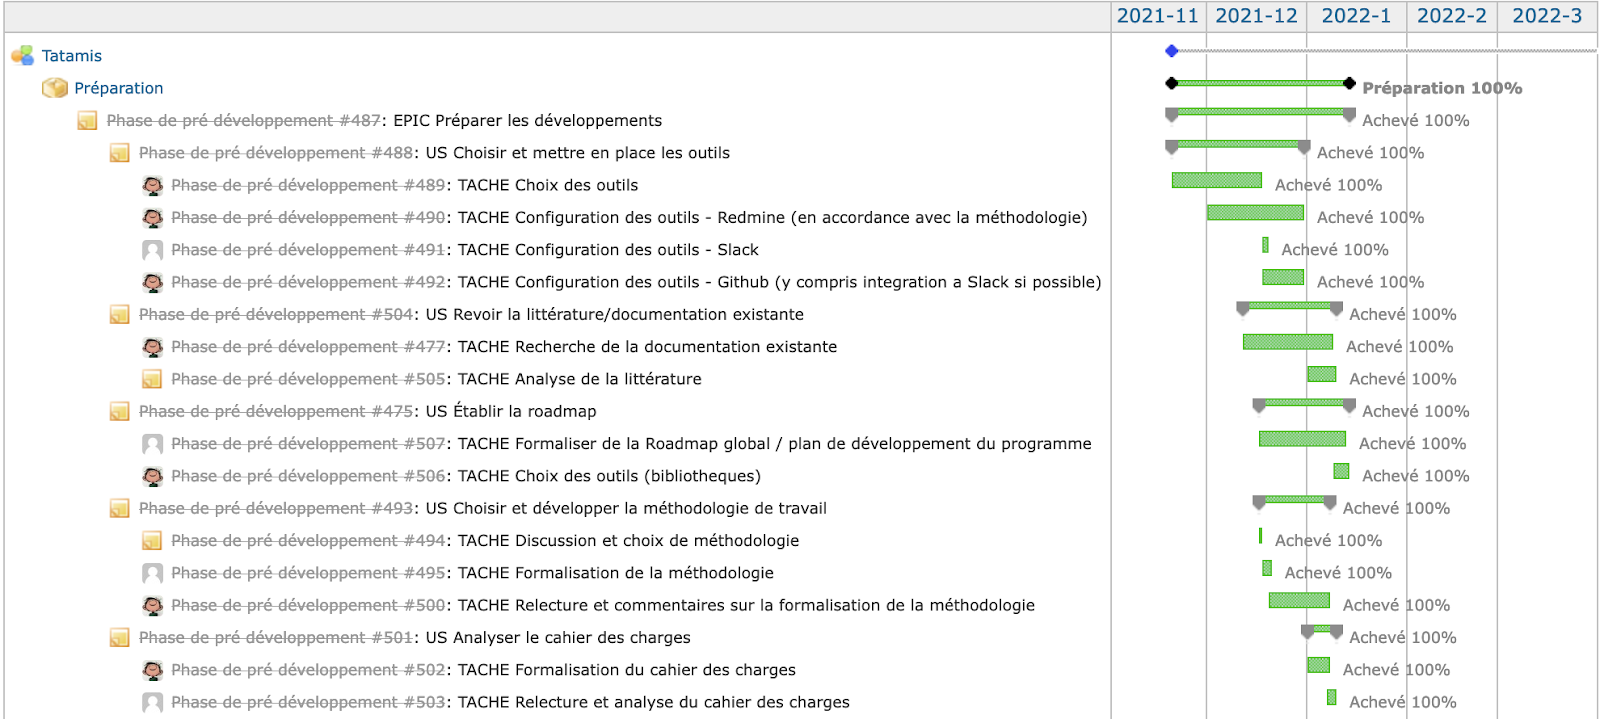
\includegraphics[width=16cm]{images/tatamis-gantt-predev.png}
\end{center}

\section{Challenges rencontrés et apprentissage}

\subsection{Challenges rencontrés et solutions appliquées}

Le principal challenge de cette phase a été de pouvoir définir une méthodologie et des méthodes d'organisation du travail alors que 
les membres de l'équipe ne se connaissent pas et n’ont pas l’habitude de travailler ensemble.
Pour réussir cette étape, nous avons essayé d’appliquer les approches suivantes:
\begin{itemize}
    \item Faire connaissance pour comprendre les forces, faiblesses et personnalités de chacun. Basé sur les expériences respectives, 
    il a paru clair que Bruno, professeur de mathématiques de profession et ayant de bonnes connaissances 
    de Python serait un atout majeur pour la partie algorithmique du projet. Benoit, responsable d’une équipe de chef de projet 
    dans le domaine informatique, serait le mieux utilisé sur des problé-matiques de gestion de projet, organisation du travail, 
    méthodologie et rédaction du rapport. Évidemment, étant bien entendu que les membres de l'équipe seront mis à contribution 
    sur tous les aspects du travail, au delà de leur domaine de prédilection
    \item Se reposer sur des méthodes de travail éprouvées, notamment par l'expérience de la gestion de projet dans le monde professionnel 
\end{itemize}

Un challenge supplémentaire a été de gérer l’absence d’un membre de l'équipe et l’incertitude liée à son implication et sa participation future.

\subsection{Apprentissage}

Le principal apprentissage est l'importance de la construction de relations pour apprendre à se connaître et travailler ensemble, 
dans le but de tirer le meilleurs des compétences de chacun des membres et de trouver un cadre de travail convenant à chacun.
